\documentclass{article}
\usepackage{epsfig}
\usepackage{times}
\usepackage{nonfloat}
\usepackage{setspace}
\usepackage[sort&compress]{natbib}
\usepackage{comment}
\usepackage[utf8]{inputenc}

\title{Appendix L: Advanced Concepts on Address Translation}
\author{Abhishek Bhattacharjee, Rutgers University}

\begin{document}

\maketitle

\section{Introduction}\label{sec:introduction}
In previous chapters, we discussed the concept of virtual memory and how modern computer architectures support it with dedicated hardware. This appendix presents a detailed treatment of this hardware support for address translation. 

As with other microarchitectural structures, address translation hardware is designed to maximize system performance and minimize power/energy consumption. However, perhaps more uniquely, address translation hardware has to balance these attributes with the need to support a programmable virtual memory interface for software developers. After all, virtual memory was originally conceived to make programming easy. It achieves this by allowing programmers to reason about how their data structures map to a flat and linear virtual address space, eschewing the complexity of the physical address space which is made up of an assortment of memory and storage devices. This separation of virtual and physical memory addresses has become so vital to the success of computing that we tend not to even think of the existence of the virtual memory abstraction when writing code today. And yet, imagine what would happen in its absence. Programmers would have to carefully reason about the capacities of device memory and storage in order to write correct code. Code written for one system would have to be refactored to port over to another system with different memory/storage configurations. Multiprogramming and security would be compromised because a program would be able to overwrite the memory image of another.  

For all these reasons, processor vendors and software developers are willing to pay an area/performance/energy "tax" to enjoy the benefits of virtual memory. This "tax" is realized in the form of dedicated address translation hardware structures like TLB structures (and other hardware) that we discuss in this appendix. Our goal is to build intuition on how best to realize this hardware in as high-performance and as energy-efficient a way as possible. A recurring theme in this appendix is our focus on real-world hardware already been built on commercial microprocessors.

\section{Address Translation on Modern Chips: An Overview}\label{sec:address-translation-on-modern-chips}

We begin with a comparison of address translation hardware available on older chips with that on available newer chips. Figure \ref{fig:address-translation-then-and-now} illustrates the evolution of address translation hardware. We refer to address translation hardware historically seen on uniprocessors in the '90s as "conventional" hardware, and contrast this against the more "modern" multi-core hardware used today.

\begin{figure}[t]
\centering
{
\begin{minipage}[t]{1.00\textwidth}
\centering
\vspace{-10mm}
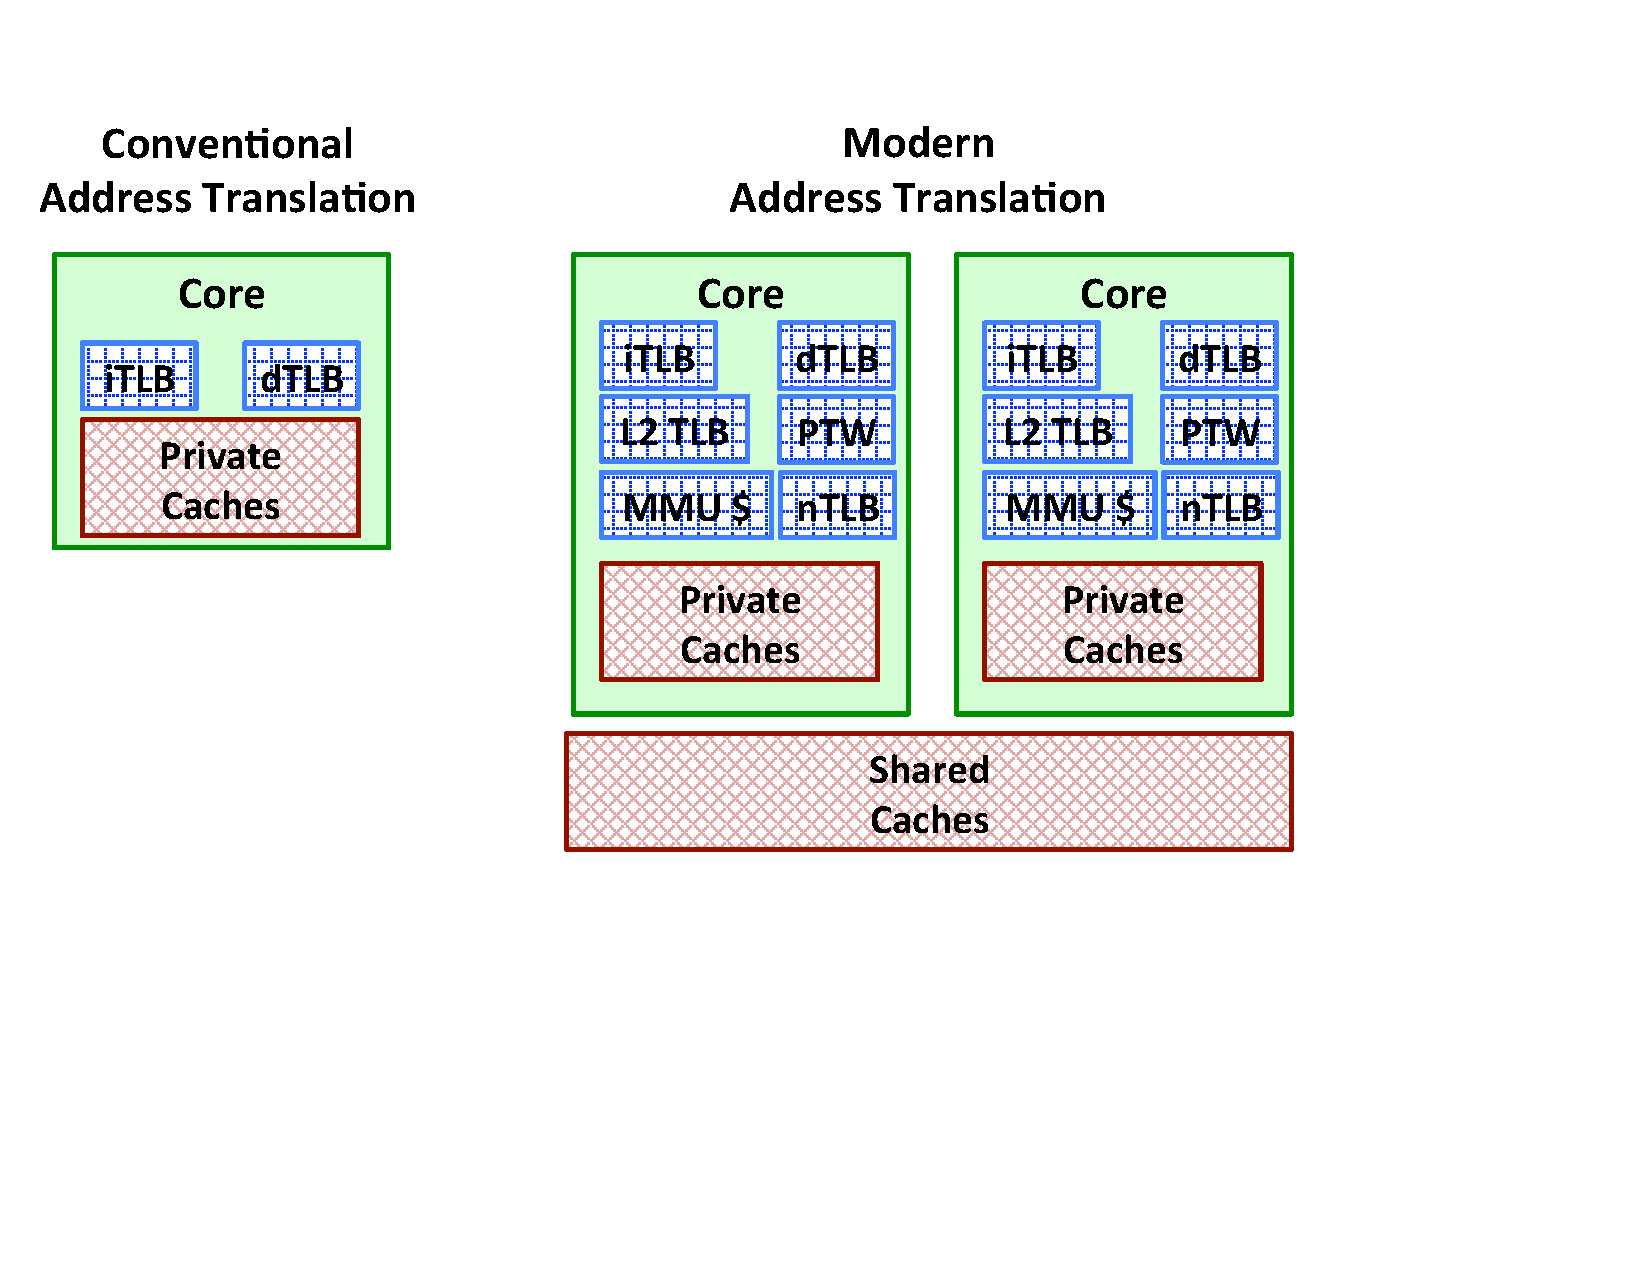
\epsfig{file=address-translation-then-and-now.pdf, scale=0.56}
\vspace{-44mm}
\caption{\small The evolution of address translation hardware from the conventional case (used circa '90s) to what is commercially available today. Address translation structures are shown in patterned blue boxes. Although private and shared caches are not dedicated address translation structures, they do cache entries from the page table.}
\label{fig:address-translation-then-and-now}
\end{minipage}
}
\end{figure}

Figure \ref{fig:address-translation-then-and-now} shows that conventionally, processor vendors have implemented split TLBs for instructions and data; i.e., iTLBs and dTLBs. Additionally, hardware caches (made up of an assortment of L1, L2, etc., caches for data and instructions) have also be used to store frequently-used entries from the page table. Unlike TLBs, in which entries store information about a single virtual-to-physical page translation, cache lines store information about multiple virtual-to-physical page translations. This is because cache lines are typically bigger than page table entries; for example, x86 systems with 64-byte cache lines typically store translations for 8 adjacent virtual pages since each page table entry is 8 bytes. Finally, an important question in address translation hardware design is the following -- who handles TLB misses when they occur? The traditional approach to this involved interrupting the operating system (OS) upon a TLB miss, at which point the OS would run a lightweight interrupt handler to "walk" the page table, find the desired page table entry, and install it in the TLB (either the iTLB or dTLB, depending on whether the memory reference was to an instruction or data).

Modern address translation hardware has come a long way since these early designs. Figure \ref{fig:address-translation-then-and-now} shows that today, we can expect to see much more sophisticated TLB hardware. Key components are:

\begin{itemize}
    \item Separate L1 TLBs for instructions and data (shown as iTLB and dTLB structures in Figure \ref{fig:address-translation-then-and-now}). Although not shown, these structures tend to be further split into separate L1 TLBs for different page sizes. As we discuss in subsequent sections, modern OSes support multiple page sizes (e.g., x86 systems support 4KB, 2MB, and 1GB pages) and it is difficult to build a set-associative L1 TLB that can concurrently support translations for multiple page sizes. 
    
    \item Unified L2 TLBs that can cache translations for instructions and data. Furthermore, modern processors occasionally support a limited set of page sizes concurrently in this L2 TLB. For example, modern Intel x86 systems implement L2 TLBs that can simultaneously support 4KB and 2MB pages, but not 1GB pages. Note that although modern L2 TLBs are unified for data and instructions, they still remain {\it private} to individual cores.
    
    \item Hardware page table walkers (PTWs) that are used to handle TLB misses {\it without} invoking the operating system. In the traditional approach without hardware PTWs, the processor must context switch the OS in on every TLB miss, interrupting user-level execution, flushing the pipeline, and polluting caches. In contrast, hardware PTWs obviate the need for all these expensive mechanisms. In fact, hardware PTWs also enable two more optimizations to hide TLB miss latencies: (1) they can overlap page table walks with independent instructions executing on the processor (as per out-of-order execution strategies like scoreboarding or Tomasulo's algorithm); and (2) they can be designed to service multiple TLB misses concurrently. 
    
    \item Memory management unit (MMU) caches that are used to accelerate TLB misses. MMU caches are a relatively new addition to the address translation hardware stack, and are targeted at x86- and ARM-style page tables. On these systems, page tables are implemented as {\it forward-mapped multi-level radix trees} rather than as linear page tables. We explain this concept and MMU caches in subsequent sections.
    
    \item Nested TLBs are specialized TLB structures aimed at supporting cloud environments running virtual machines. Since these environments suffer from particularly high address translation overhead, processor vendors build dedicated TLBs to support their complex page table structures. We discuss this further in subsequent sections.
    
    \item Hardware caches continue to support, similar to the conventional address translation case, page table entry caching. However, some architectures like Sparc develop the design of special software structures called {\it Translation Storage Buffers} for use in the hardware caches. 
    
\end{itemize}

While the particular configuration parameters of these parts of the address translation stack can vary across architectures, we provide some insight on their relative sizes, latencies, etc., by summarizing their parameters on Intel's Skylake chip. Figure \ref{fig:skylake-parameters} quantifies the capacities, organizations, and access latencies of the various system TLBs, hardware page table walkers, MMU caches/nested TLBs. The remainder of this appendix is dedicated to performing a deep dive on each of these hardware structures.

\begin{figure}[t]
\centering
{
\begin{minipage}[t]{1.00\textwidth}
\centering
\vspace{-10mm}
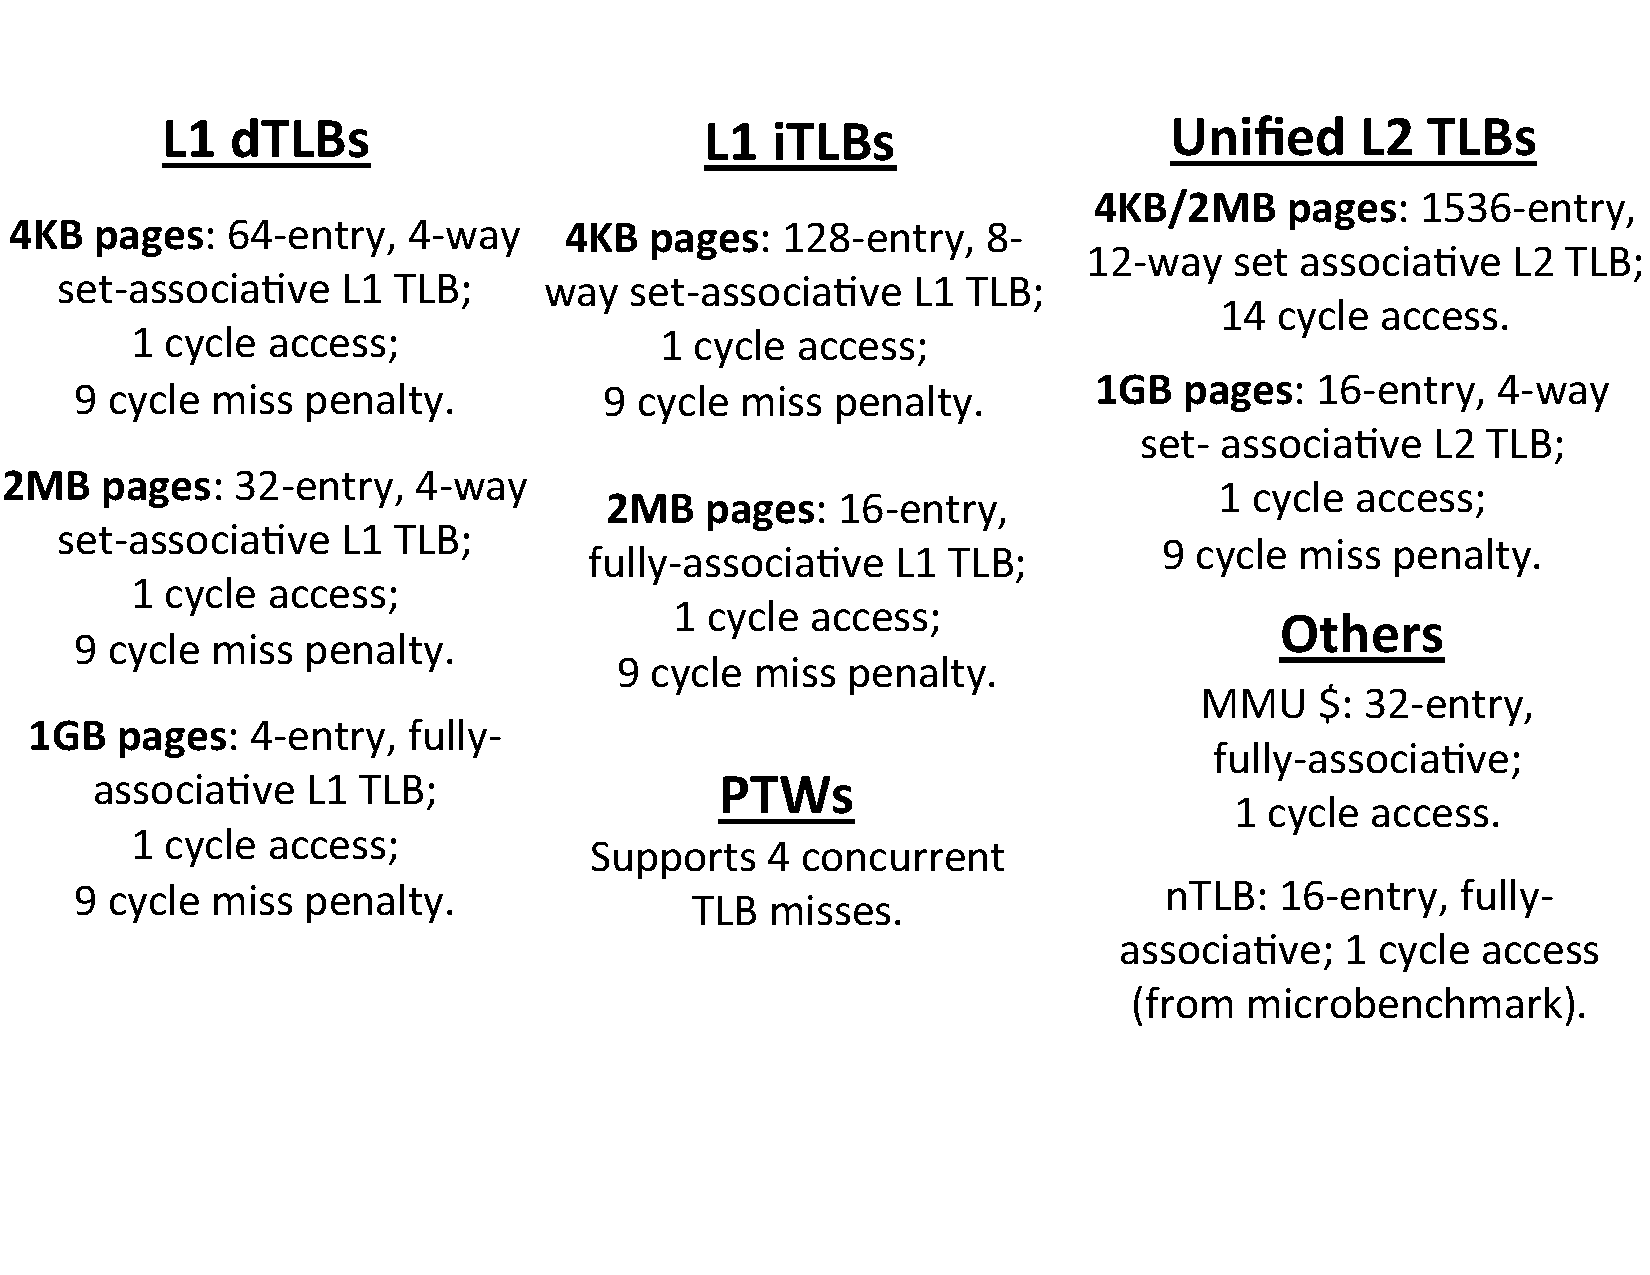
\epsfig{file=skylake-parameters.pdf, scale=0.45}
\vspace{-24mm}
\caption{\small Parameters of the addess translation hardware available on Intel's Skylake chips as of 2018. While the parameters of most of these hardware structures are public, the nested TLB sizes are inferred based on experiments we ran using microbenchmarks designed to identify capacity and associativity.}
\label{fig:skylake-parameters}
\end{minipage}
}
\end{figure}

\section{Split L1 TLBs}\label{sec:split-l1-tlbs}

Modern processors implement a group of split L1 TLBs for instructions and data, separated by page size. The rationale for both is the following:

\vspace{2mm}
{\noindent \bf Why implement separate instruction and data L1 TLBs?} There are several reasons that processor vendors opt to employ separate L1 TLBs for instructions and data. First, modern superscalar out-of-order pipelines can require several concurrent instruction and data virtual-to-physical translations per cycle. In this context, implementing separate iTLBs and dTLBs reduces the chances of pipeline hazards due to contention at the TLB from limited port count, etc. Second, instructions and data exhibit vastly different locality of reference or reuse attributes. For example, it is well known that programs generally have much smaller portions of their memory footprint dedicated to instructions than to data. At the same time, instruction references are more "critical" to performance; i.e., while data references can generally be overlapped by independent streams of instructions because of out-of-order capabilities, instruction references are often on the critical path of performance. Therefore, TLB misses for instructions can have a particularly pernicious impact on performance. For these reasons, it is difficult -- although not impossible -- to design a single TLB structure with the appropriate replacement/allocation policy to manage the needs of instruction and data references. Consequently, processors vendors opt for separate iTLBs and dTLBs. 

One implication of split L1 TLBs is that vendors can use different policies among the TLB resources when supporting hyperthreading. For example, because of the criticality of instruction references to overall performance, processor vendors typically implement statically partitioned iTLBs for hyperthreads. Consider, for example, Intel's Skylake architecture, where the 128-entry L1 iTLBs are statically partitioned across the two threads when two-way hyperthreading is enabled. In this case, each thread is guaranteed 64 instruction TLB entries, preventing fairness problems that would arise in a dynamically partitioned scheme if one thread had a bigger instruction footprint than the other. In contrast, dTLBs are typically partitioned dynamically among hyperthreads. The rationale is that different threads may have different memory footprints dedicated to their heaps/stacks, and adapting a common pool of TLB resources dynamically among the competing threads may make better overall use of the structure. For this reason, Intel's Skylake architecture, for example, dynamically partitions the L1 dTLB among hyperthreads.

\vspace{2mm}
{\noindent \bf Why implement separate L1 TLBs for different page sizes?} L1 TLBs must be high performance and energy-efficient. Performance is desirable as TLBs reside on the timing-critical L1 datapath of pipelines. This means that they are usually built in a simple manner that easily meets timing constraints, with lookup and miss handling properties that are amenable to speed. Additionally, energy-efficiency is desirable as TLBs can consume a significant amount -- as much as 15\% -- of processor energy. 

These two design targets generally mean that L1 TLBs are realized with set-associa\-tive RAM or CAM structures. However, set-associativity poses correctness challenges with respect to large pages or superpages. Large pages are commonly employed by most OSes today. The motivation for large pages is that they enable greater effective TLB capacity -- for example, a single TLB entry on x86 systems can support a 4KB page but with large page support, the same entry can be used to support a 2MB or 1GB large page instead. Large pages can dramatically reduce the frequency of TLB misses.

However, supporting multiple page sizes also complicates the design of set-associat\-ive TLBs. The reason is that different page sizes require a different number of page offset bits. For example, on x86 systems, 4KB baseline pages require 12 page offset bits, 2MB large pages require 21 page offset bits, while 1GB large pages require 30 page offset bits. 



\section{Unified L2 TLBs}\label{sec:unified-l2-tlbs}

\section{TLB Prefetching}\label{sec:tlb-prefetching}

\section{TLB Coherence}\label{sec:tlb-coherence}

\section{Multiple Page Size Support and Coalescing}\label{sec:tlb-multiple-page-size-coalescing}

\section{Page Table Walkers}\label{sec:page-table-walkers}

\section{Memory Management Unit Caches}\label{sec:mmu-caches}

\section{Nested TLBs}\label{sec:ntlbs}

\section{Hardware Caches and Translation Storage Buffers}\label{sec:hw-caches-tsbs}

\section{Future Designs: Shared Last-Level TLBs}\label{sec:future-designs-shared-tlbs}

\end{document}
